\documentclass[12pt,a4paper]{article}
%usepackage[spanish]{babel}
\usepackage[spanish,es-tabla]{babel}
\usepackage[utf8]{inputenc}
\usepackage{amsmath}
\usepackage{amsfonts}
\usepackage{amssymb}
\usepackage{graphicx}
\usepackage{natbib} % Para detates de citacion
\usepackage[section]{placeins}
\usepackage[table,xcdraw]{xcolor}
\usepackage{graphicx}
\usepackage{caption}
\usepackage{url}
\usepackage[pangram]{blindtext} % Solo genera texto aleatorio


\author{Abel E. Cuevas Jiménez \\ Mario A. Lopez Alvarado \\ Jesús Márquez Avilés} % \\ Salto de línea
\title{\bf{Análisis estadístico para una campaña de vacunación contra el COVID-19 }}
\begin{document}

\begin{titlepage}
\centering
{\includegraphics[width=0.25\textwidth]{unam.jpg}\par}
\vspace{0.5cm}
{\bfseries\LARGE Universidad Nacional Autónoma de México \par}
\vspace{.5cm}
{\scshape\Large Centro de Nanociencias y Nanotecnología \par}
\vspace{2.5cm}
{\scshape\Huge Análisis estadístico para una campaña de vacunación contra el COVID-19 \par}
\vspace{2.5cm}
{\itshape\Large Proyecto final de Probabilidad y Estadística \par}
\vfill
{\Large Autores: \par}
{\Large \\Mario Alejando López Alvarado\\ Jesús Márquez Avilés\\ Abel Emiliano Cuevas Jiménez\par}
\vfill
{\Large 03 de febrero de 2021 \par}
\end{titlepage}


\newpage
\tableofcontents
%%\maketitle
\newpage


%%%%%%%%%%%%%%%%%%%%%%%% Empieza Integrantes %%%%%%%%%%%%%%%%%%5
\section{Trabajo de los integrantes}
\setlength{\parindent}{0cm}
Todos los miembros del equipo aportaron de forma equitativa al trabajo.
\setlength{\parindent}{1cm}
%%%%%%%%%%%%%%%%%%%%%%% Termina integrantes %%%%%%%%%%%%%%%%%%%%%%%%

%%%%%%%%%%%%%%%%%% Empieza motivación %%%%%%%%%%%%%%%%%%%%%

\section{Motivación}

\setlength{\parindent}{0cm}
Dada la situación en la que el mundo se encuentra, la información es la única manera de poder vislumbrar la luz al final del camino, el COVID-19 deja un mar de preguntas sobre la manera de actuar tanto de la gente, como de los gobiernos. Nuestra motivación para realizar este trabajo es averiguar quiénes de nuestros seres queridos o de la misma población mexicana se encuentra en mayor riesgo, para así poder proponer una campaña de vacunación, basándose enteramente en la vulnerabilidad de la población.
\setlength{\parindent}{1cm}

%%%%%%%%%%%%%%% Termina motivacion %%%%%%%%%%%%%%%%%%%%%%%%%%%%

%%%%%%%%%%%%%% Empieza Introduccion %%%%%%%%%%%%%%%%%%%%%%%%%%
\section{Introducción}
\setlength{\parindent}{0cm}


Actualmente México se encuentra bajo los efectos de una emergencia sanitaria causada por el virus SARS-CoV-2, lo que ocasiona muertes a lo largo de los diferentes grupos de edad en la población mexicana, la cual, según el censo del 2015, está distribuida como se observa en la tabla \ref{edades} \citep{INEGI}. \\ Tanto en la campana de población mexicana como en la tabla 1, se puede observar que existe un menor número de personas de la tercera edad (60 años en adelante) que personas jóvenes.

\begin{center}
    \captionof{table}{Población mexicana según grupos de edad\label{edades}}
    \begin{tabular}{|c|c|c|c|c|}
\hline
\rowcolor[HTML]{C0C0C0} 
\multicolumn{1}{|c|}{\cellcolor[HTML]{C0C0C0}\textbf{Edad}}      & 0-9        & 10-19      & 20-29      & 30-39      \\ \hline
\multicolumn{1}{|c|}{\cellcolor[HTML]{C0C0C0}\textbf{Población}} & 21,523,328 & 22,000,529 & 19,918,412 & 17,540,189 \\ \hline
\rowcolor[HTML]{C0C0C0} 
\cellcolor[HTML]{C0C0C0}\textbf{Edad}                                     & 40-49      & 50-59      & 60-69      & 70+        \\ \hline
\cellcolor[HTML]{C0C0C0}\textbf{Población}                                & 15,023,137 & 11,002,068 & 6,877,071  & 5,559,250  \\ \hline

\end{tabular} 
\end{center}
A la población constantemente se le está realizando pruebas para estimar el número de contagiados por la COVID-19 y existen tres formas de dictaminar que un individuo es positivo a enfermedad, la primera es al ser confirmado por asociación lo cual aplica cuando el caso informó ser contacto de un positivo a COVID-19 (y este se encuentra registrado en el Sistema de Vigilancia Epidemiológica de Enfermedades Respiratorias ó \textit{SISVER}) y al caso no se le tomó muestra o esta resulto no valida, la segunda es al ser confirmado por dictaminación, lo cual solo aplica para defunciones de casos
que no se le tomo muestra o sí se tomó muestra, pero la muestra resultó no válida y por último, el ser confirmado por muestra de laboratorio o prueba antigénica. \citep{ss} \\

El gobierno de México, y la \textit{OMS} (Organización Mundial de Salud), reportan un mayor riesgo de muerte mientras la edad del paciente con COVID-19 aumenta. Es por esto que el gobierno mexicano planteo en su jornada de vacunación seguir con las personas mayores de 80, después de los trabajadores de salud y terminar la jornada con personas menores a 40 años \citep{GTAV}.

\setlength{\parindent}{1cm}

%%%%%%%%%%%%%%%%%%%%%%%%% Termina introducción %%%%%%%%%%%%%

\section{Hipótesis}
\begin{enumerate}
  \item A medida que la edad de la población aumente, se observará mayor vulnerabilidad ante la COVID-19.
  \item En rangos de 20 a 40 años, se observará mayores contagios.
  \item No se tendrá que vacunar a toda la población para que baje la mortalidad del pueblo mexicano por el SARS-CoV-2, es decir, se logrará una "inmunidad de rebaño" una vez que haya una gran cantidad de vacunados.
\end{enumerate} 




\section{Metodología}
\subsection{Búsqueda de datos}
\setlength{\parindent}{0cm}
Para este estudio se usó como referencia el censo del INEGI del 2015 para obtener datos de la población total mexicana por rango de edades \citep{INEGI}. Por otro lado, se usaron los datos abiertos del COVID-19 de la Secretaria de Salud actualizados hasta el 21 de enero de 2021 \citep{ss}.
\setlength{\parindent}{1cm}

\subsection{Análisis}
\setlength{\parindent}{0cm}
Con ayuda del programa \texttt{ACCESS} de \textit{Microsoft} y lenguaje \texttt{SQL}, se filtraron los datos de COVID para el uso exclusivo de aquellos en que su clasificación final fue de: (1) caso de COVID-19 confirmado por asociación clínica epidemiológica; (2) caso de COVID-19 confirmado por comité de dictaminación; (3) Caso de SARS-COV-2 confirmado. A partir de ellos, se extrajo la fecha de defunción; edad; mujeres embarazadas; personas con diabetes, EPOC, asma, inmunosupresión, hipertensión, enfermedades cardiovasculares, obesidad, enfermedad renal crónica, y otras comorbilidades; personas con tabaquismo; aquellas personas que fueron intubadas y las que presentaron neumonía.  
\\ 
Una vez que los datos fueron filtrados, se exportaron a un documento \texttt{.csv} delimitado por comas para su uso en \texttt{Matlab}, donde se modeló el número de muertes confirmadas por rango de edades y la curva de contagio por días de la población general y por rango de edades. 
\setlength{\parindent}{1cm}

\subsection{Sistema de puntaje}
\setlength{\parindent}{0cm}
Se estableció un porcentaje de relación entre las personas que mueren y aquellas que tienen una enfermedad o complicación específica (\textit{ECE}). 
\begin{equation}\\
\frac{Muertos\;por\;COVID-19\;con\;una\;ECE}{Total\;de\;personas\;con\;una \;ECE}= \%\;de\;relación
\end{equation}
Las enfermedades o complicaciones que tuvieron un mayor porcentaje tendrán un mayor puntaje. 
Reescrito de otra forma: 
\begin{equation}
    \frac{nm_e}{N_e} =r_i
\end{equation}

Donde \textit{nm} es el número de muertos por COVID-19 de una \textit{ECE} total de la población,  \textit{Ne} el número de enfermos total de la población de una sola \textit{ECE} y \textit{r }el porcentaje de relación. 
\\
Para determinar el puntaje \textit{p} de cada \textit{ECE} se usó lo siguiente: 
\begin{equation}
    p_i=\frac{r_i}{\mathrm{\Sigma}r_i}\cdot\ c
\end{equation}
Donde \textit{c} es una constante para ajustar el número de dígitos antes o después del cero. 

Posteriormente para determinar el puntaje \textit{P} para cada rango de edad \textit{E} por una sola \textit{ECE}  se usó: 
\begin{equation}
    P_{ECE}^E=p_iN_{ECE}^E
\end{equation}
Donde \(N_{ECE}^E\) es el número de enfermos de una enfermedad \textit{ECE} de un rango de edad \textit{E}  
\\
Finalmente, el puntaje total \(P_T^E\) para un rango de edad fue: 
\begin{equation}
    P_T^E=\mathrm{\Sigma}\ P_{ECE}^E
\end{equation}
\setlength{\parindent}{1cm}

\subsection{Puntos de equilibrio}
\setlength{\parindent}{0cm}
Los puntos de equilibrio se determinan a partir de una probabilidad de muerte que sea menor o igual a \textit{p} para cada rango de edad. Donde \textit{p} es una probabilidad propuesta de manera arbitraria. El resultado será un número de personas por rango de edad que se deben vacunar como MÍNIMO (con respecto a \textit{p}) para pasar al siguiente rango de edad para vacunación. 
\\ 
Si se toma como una muestra los datos de COVID-19 del gobierno, se puede inferir que la población tendrá el mismo comportamiento. 
\\ 
Con el uso de la base de datos gubernamental y bajo la priorización de las personas que mueren a causa del virus, se calculó primero el porcentaje de muertos \textit{m} para cada rango de edad \textit{E} que se encuentra contagiada: 
\begin{equation}
    m^E=\frac{nm^E}{Nc^E}
\end{equation}
Donde \(nm^E\) es el número de muertos por rango de edad y  \(Nc^E\) es el número de contagiados por rango de edad.
\\
La mortalidad \textit{m} de la muestra se acerca a la mortalidad \textit{M} de la población.
\begin{equation}
    m\simeq M
\end{equation}
Entonces, para una población total \(N_p^E\) para cada rango de edad tendremos una mortalidad asociada \(M^E\). El valor esperado para el número de muertos total en caso de que toda la población se contagie bajo las mismas condiciones que la muestra se define de la siguiente forma: 
\begin{equation}
    E\left(N_p^E\right)=m^EN_p^E=X
\end{equation}
No obstante, cada que se toma una muestra sin reposición \(n=\left[N_1,N_2,N_3\ldots\right]\)con la misma probabilidad \(M^E\), se tiene una nueva mortalidad \(M_i^E\) en la población: 
\begin{equation}
    M_i^E=\frac{X_i}{N_p^E}
\end{equation}
Donde \(X_i=m^EN_p^E-\left(i-1\right)m^En\); y \textit{n} es el tamaño de la muestra. 
\\
Cabe resaltar que cuando \(i=\frac{N_p^E}{n}+1\); \(M_i^E=0\). Sin embargo, nos limitamos a llegar al punto de equilibrio donde:  
\begin{equation}
    M_i^E\le p
\end{equation}
\setlength{\parindent}{1cm}


\section{Resultados y Discusión}

\subsection{Estadísticas de mortalidad para el COVID-19 en México}
\setlength{\parindent}{0cm}
El primer análisis realizado fue un estudio estadístico de la mortalidad por la enfermedad COVID-19 (obsérvese figura \ref{Figura1}), según los distintos grupos de edad reportados en el censo poblacional antes mencionado. \\
\begin{figure}
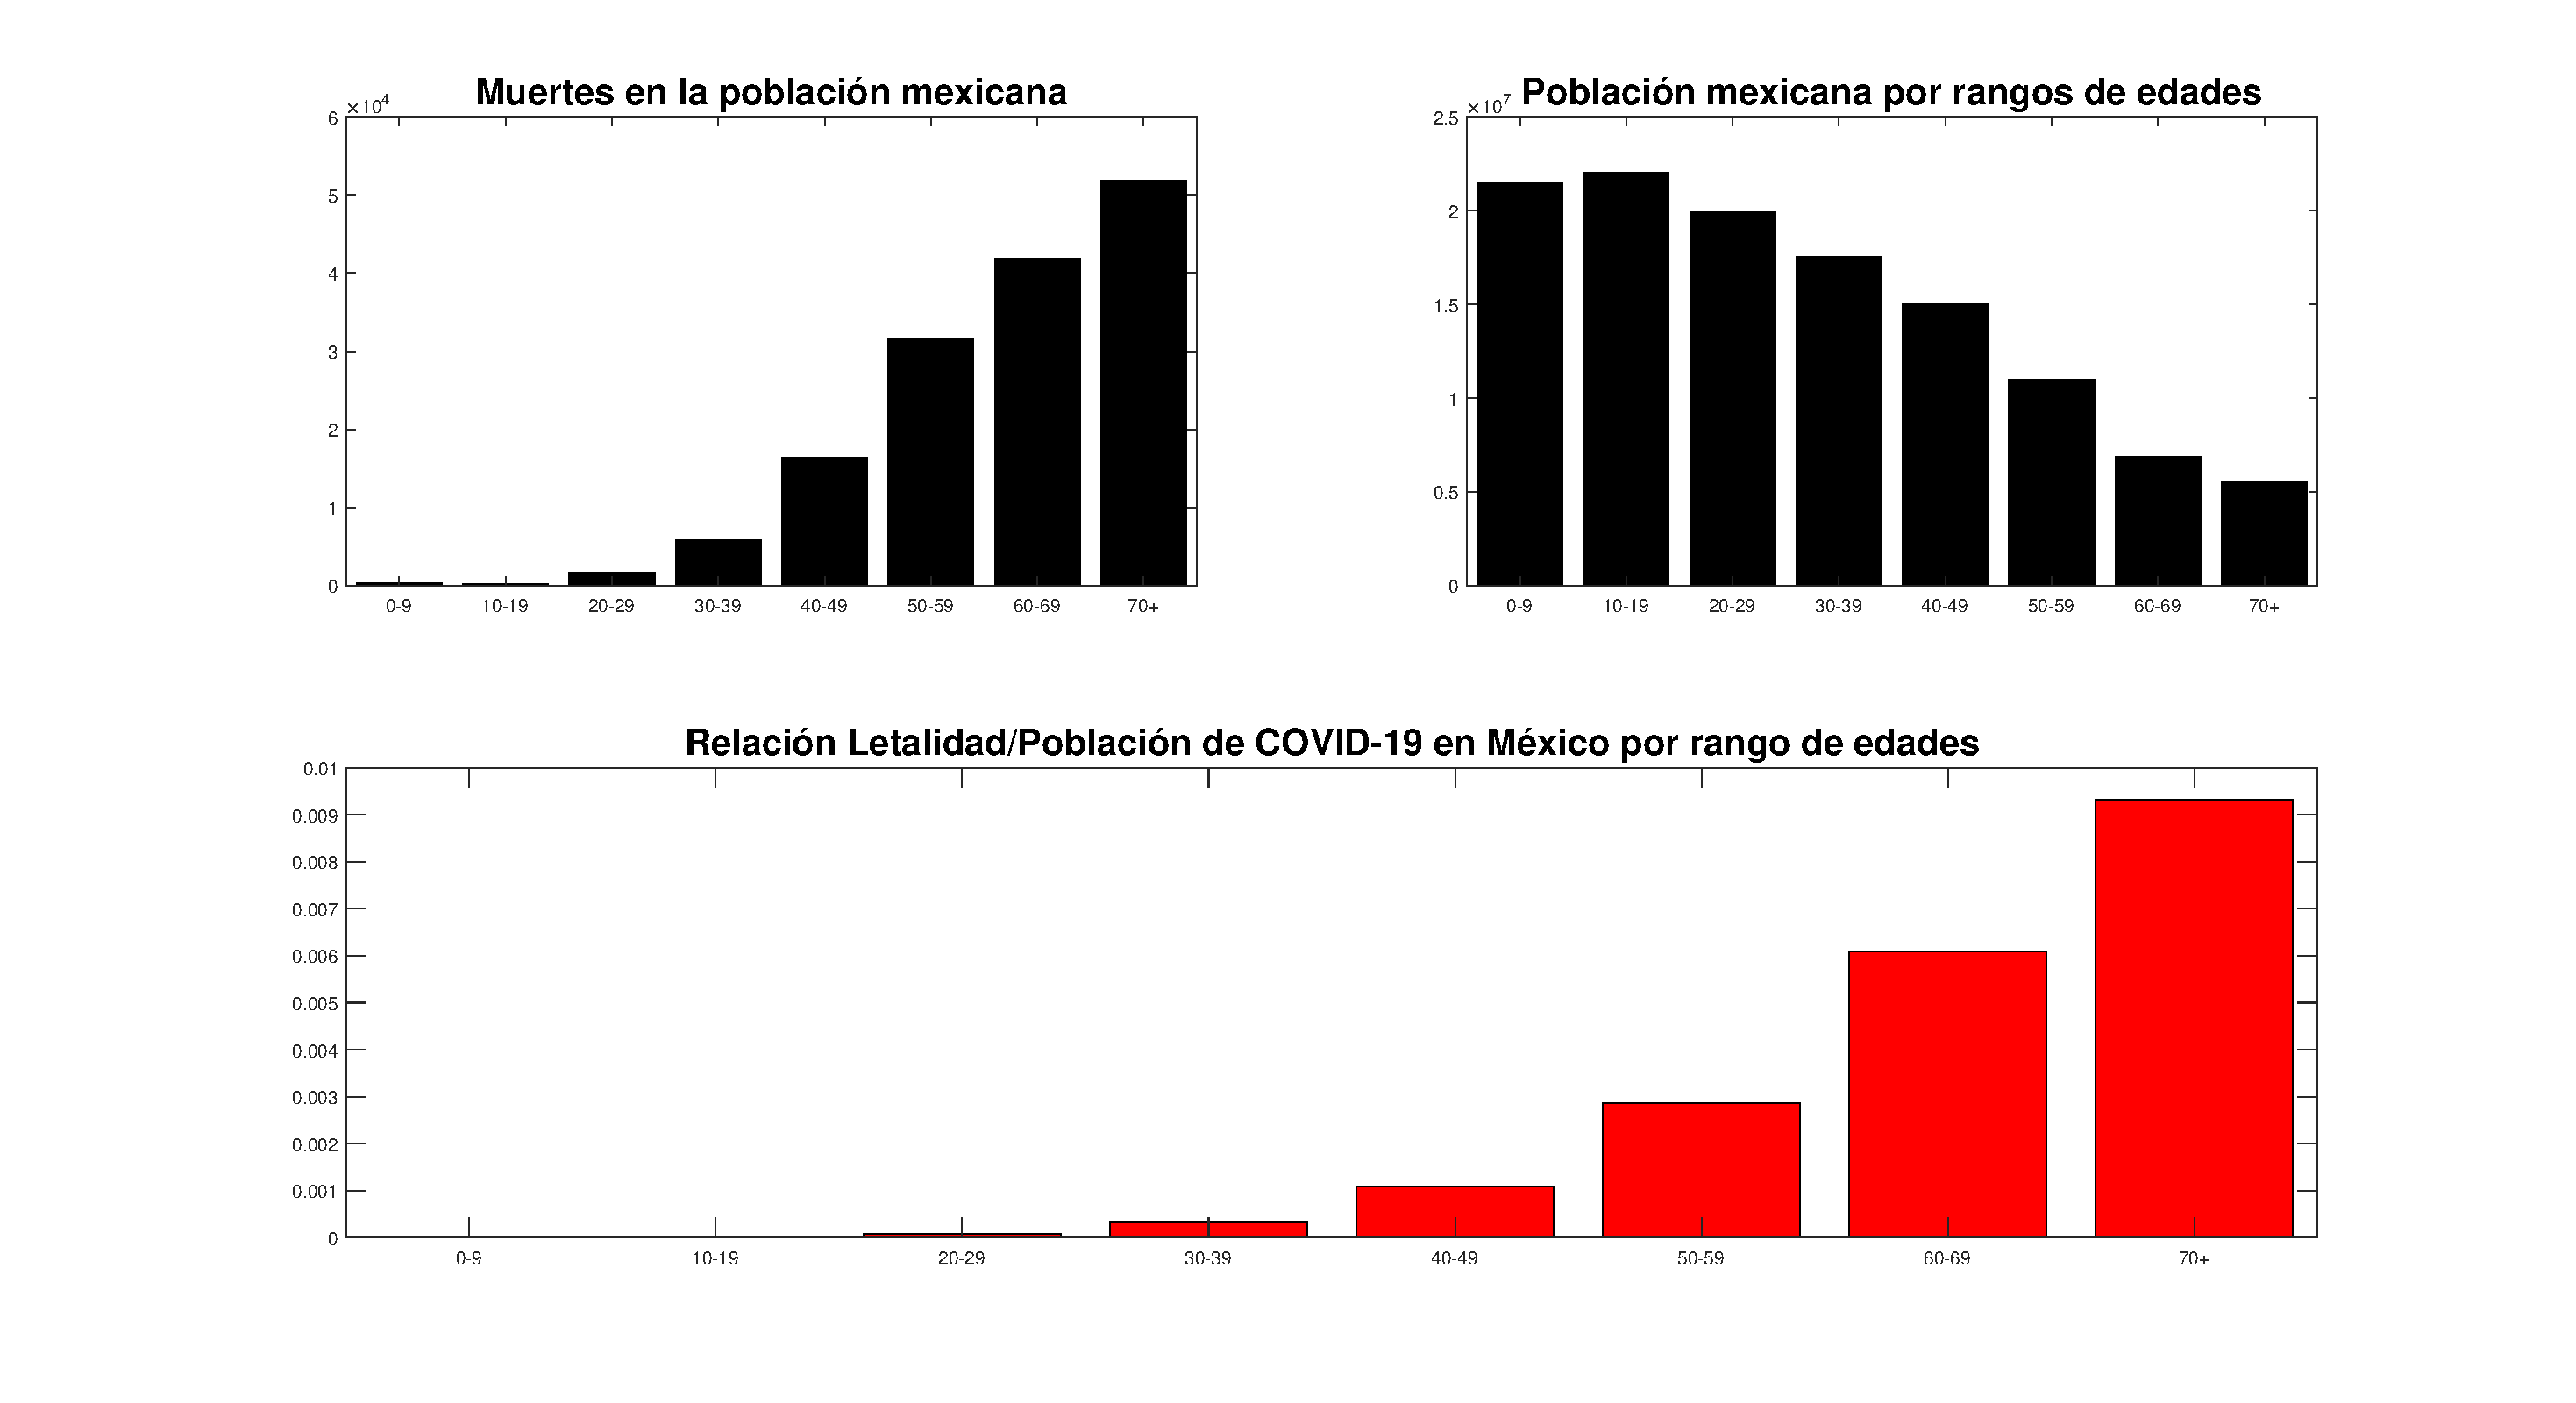
\includegraphics[width = 0.9\textwidth]{Figura1.eps}
\centering
\caption{Gráficos de estadísticas relacionadas al COVID-19 en México} \\
\label{Figura1}
\end{figure}

En la primera gráfica se demuestra lo reportado por la OMS, es decir, a medida que la edad del paciente es mayor, el riesgo de muerte por COVID-19 aumenta. Al comparar estos datos con el número de habitantes por rango de edad en México, se observa también que los rangos de edad más propensos a morir son justamente los que poseen menor población (véase figura 1b). Al realizar un cociente entre ambos datos obtenemos la gráfica que se observa en la figura 1c, simbolizando el nivel de vulnerabilidad a la enfermedad tomando en cuenta únicamente el número de muertes y el tamaño de la población en dicho rango de edad.  
\setlength{\parindent}{1cm}

\subsection{Curvas de contagio según grupos de edades}
\setlength{\parindent}{0cm}

Para estudiar la propagación de la enfermedad en la población mexicana por grupos de edad, se generó una curva de contagio a través del tiempo (día por día) para cada rango de edad (véase figura \ref{Figura2}). \\
\begin{figure}
\centering
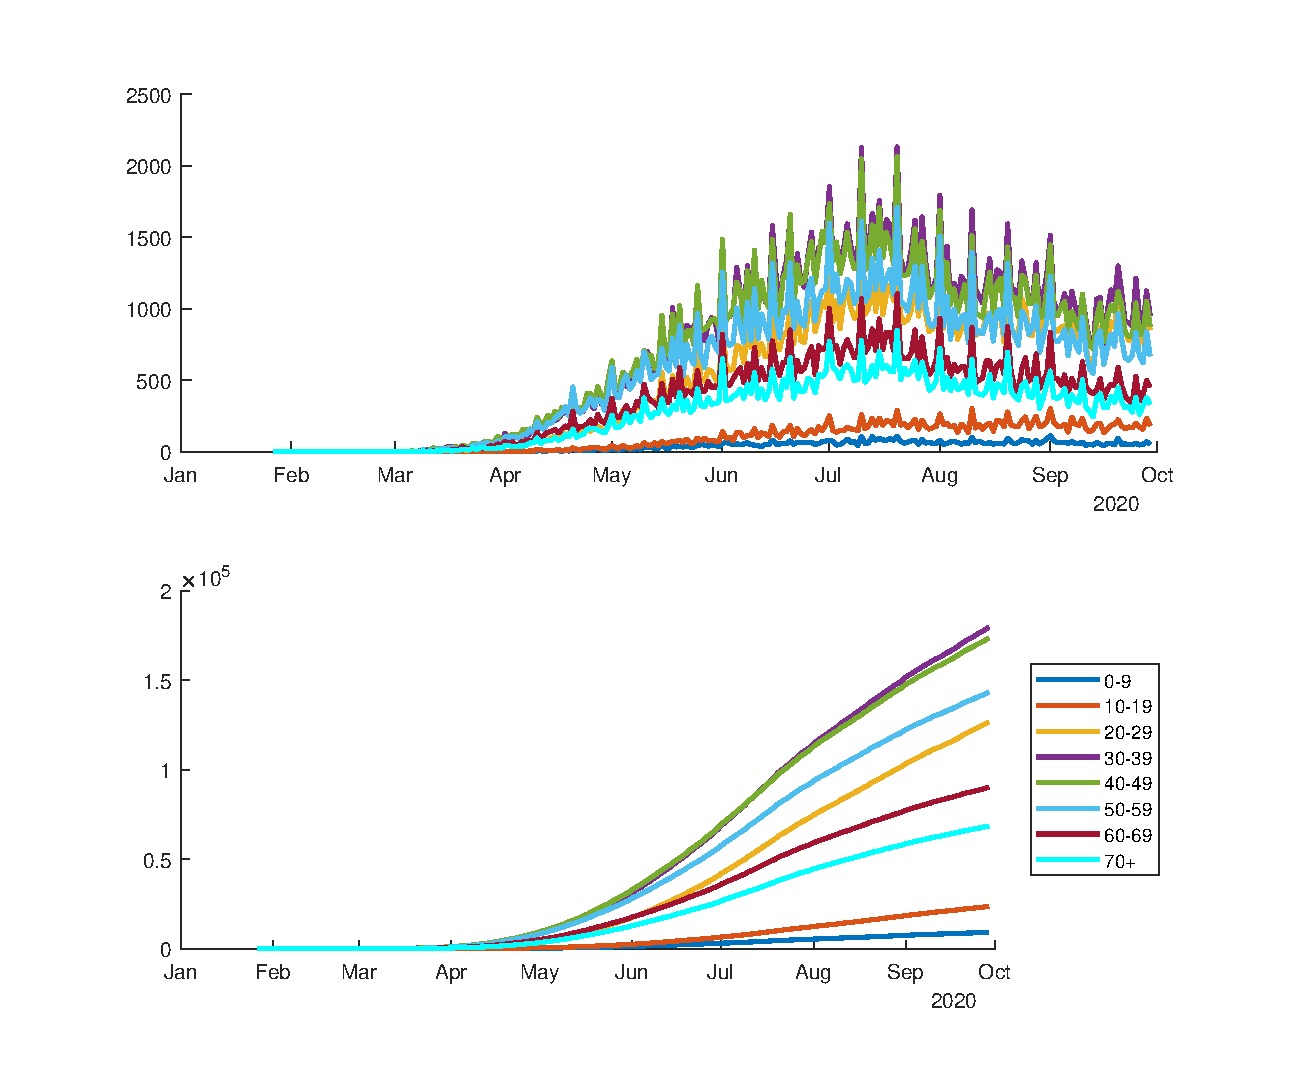
\includegraphics[width = 0.8\textwidth]{Figura2.eps}
\caption{Curvas de contagio por COVID-19 según rangos de edad en México} \\ 
\label{Figura2}
\end{figure}

En la figura 2a se observan los contagios por día para un grupo de edad específico, mientras que en la figura 2b se observan los contagios acumulados a través del tiempo. Algo importante de resaltar de estos datos, es el hecho de que los rangos de edad de entre 30 y 49 años son los más contagiados. Esto es coherente a la situación actual en México, donde justamente este rango de edad pertenece a la clase trabajadora del país y, por lo tanto, se ve expuesta en gran medida al virus debido a que es forzada a salir de su casa para laborar.\\

Por otro lado, el rango de edad de 70 años o más se encuentra bastante bajo en el número de contagios tanto acumulados como en diarios, esto puede deberse a la vulnerabilidad de este sector de la población, es decir, como son propensos a complicaciones mantienen su sana distancia e intentan no salir de casa y en general tienen mayor precaución.
\setlength{\parindent}{1cm}

\subsection{Puntaje de complicaciones para el COVID-19 (Neumonía e Intubación)}
\setlength{\parindent}{0cm}
Se utilizó la ecuación 2 para calcular el porcentaje de personas que morían cuando sufrían neumonía o una intubación (ver tabla \ref{puntaje1})

\begin{center}
    \captionof{table}{Porcentaje de muertes por complicación\label{puntaje1}}
    \begin{tabular}{|c|c|c|}
\hline
\rowcolor[HTML]{C0C0C0} 
\textbf{Complicación}                                      & Neumonía & Intubado \\ \hline
\cellcolor[HTML]{C0C0C0}\textbf{Porcentaje de muerte (\%)} & 42.25    & 80.86    \\ \hline
\end{tabular} 
\end{center}
Como se observa en la tabla, es más probable morir cuando se es intubado, esto lo podemos relacionar con el estado en el que las personas llegan a requerir la intubación, es decir, las personas que necesitan de este servicio se encuentran en un estado crítico de salud.\\
Siguiendo con la sección 5.3, se obtuvo la figura \ref{Figura3}, en esta se puede observar que a medida que el rango de edad sube, aumenta el puntaje (histograma azul), siendo el rango de 70+ el de mayor puntuación. 

\begin{figure}
\centering
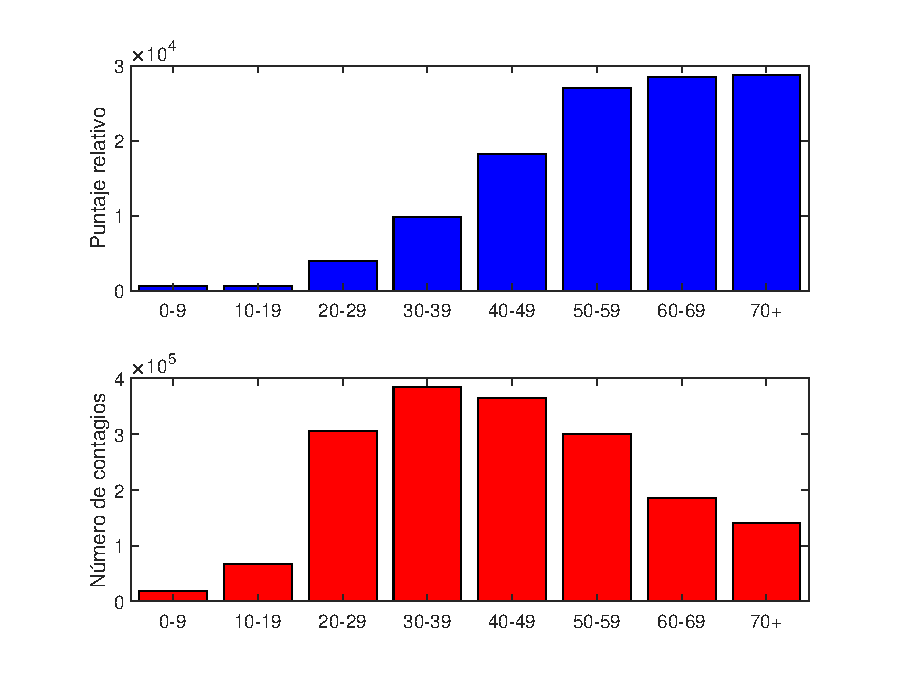
\includegraphics[width = 0.8\textwidth]{Figura3.eps}
\caption{Sistema de puntaje relativo para complicaciones del COVID-19}  
\label{Figura3}
\end{figure}

Además se observa que la población económicamente activa (20-59 años), en su mayoría tienen una puntuación baja pero un alto número de contagios; cabe recalcar que el rango de 50-59 años tienen un número de contagios relativamente alto además de un alto riesgo de sufrir una complicación (puntuación alta). 
\setlength{\parindent}{1cm}

\newpage
\subsection{Puntaje de comorbilidades para población infectada con COVID-19}
\setlength{\parindent}{0cm}

De forma similar a la sección 6.3, se usó la ecuación 2 para calcular la relación entre la muerte por COVID-19 y las diferentes comorbilidades de las personas (ver tabla \ref{puntaje2}). 
\begin{center}
    \captionof{table}{Porcentaje de muerte por comorbilidad\label{puntaje2}}
   \begin{tabular}{|
>{\columncolor[HTML]{C0C0C0}}c |
>{\columncolor[HTML]{FFFFFF}}c |}
\hline
\textbf{Comorbilidades}                                                                         & \cellcolor[HTML]{C0C0C0}\textbf{\begin{tabular}[c]{@{}c@{}}Porcentaje \\ de muerte (\%)\end{tabular}} \\ \hline
\cellcolor[HTML]{C0C0C0}Asma                                                                    & 6.84                                                                                                  \\ \hline
\cellcolor[HTML]{C0C0C0}\begin{tabular}[c]{@{}c@{}}Enfermedades\\ cardiovasculares\end{tabular} & 27.14                                                                                                 \\ \hline
\cellcolor[HTML]{C0C0C0}Obesidad                                                                & 12.85                                                                                                 \\ \hline
EPOC                                                                                            & 33.64                                                                                                 \\ \hline
\cellcolor[HTML]{C0C0C0}Diabetes                                                                & 23.76                                                                                                 \\ \hline
\cellcolor[HTML]{C0C0C0}Hipertensión                                                            & 22.01                                                                                                 \\ \hline
Inmunosupresión                                                                                 & 22.05                                                                                                 \\ \hline
\begin{tabular}[c]{@{}c@{}}Enfermedad\\ renal crónica\end{tabular}                              & 39.13                                                                                                 \\ \hline
Tabaquismo                                                                                      & 8.94                                                                                                  \\ \hline
\begin{tabular}[c]{@{}c@{}}Otra \\ comorbilidad\end{tabular}                                    & 22.63                                                                                                 \\ \hline
\end{tabular}
\end{center}\\

La relación más fuerte entre la muerte por COVID-19 y alguna comorbilidad se observa para la enfermedad renal crónica, EPOC y enfermedades cardiovasculares. Por otro lado, el riesgo asociado para el asma y el tabaquismo permanece bajo respecto a los demás a pesar de su implicación negativa en las vías respiratorias.  

\\Igual que en la sección anterior se compararon los puntajes con los números de contagios por rango de edad y se obtuvo la figura \ref{Figura4}, se observa que el rango de edad de 50 a 59 son los que mayor puntaje tienen, denotando que son los que cuentan con más comorbilidades.

\begin{figure}
\centering
\includegraphics[width = 0.8\textwidth]{Figura4.eps}
\caption{Sistema de puntaje de morbilidades según grupos de edad}  \\
\label{Figura4}
\end{figure}
Se puede observar que existe un declive en el puntaje después de los 59 años, probablemente esto se puede deber a que las personas que tienen tantas comorbilidades normalmente no llegan a la tercera edad.\\
También, se puede comparar la figura \ref{Figura4} con la figura \ref{Figura3} se observa que los que más sufren complicaciones y los que tienen una mayor comorbilidad son el mismo sector de población, las personas de 50 a 59 años, además estos tienen un alto porcentaje de contagio. \\


Idealmente, las campañas y medidas preventivas deberían estar enfocadas a los rangos de edades que tengan un mayor puntaje relativo; no obstante, la priorización debe ser en aquellos que tengan las enfermedades o comorbilidades mayormente relacionadas con la muerte por COVID-19.  
\setlength{\parindent}{1cm}
\subsection{Propuesta de campaña de vacunación}
\setlength{\parindent}{0cm}
Para poder proponer una campaña de vacunación con una fecha estimada en la que deberá completarse, se asumió que se iniciará con un total de 1 millón de vacunas. Se propuso también que cada mes este número aumentaría por 500,000 vacunas hasta llegar a un total de 4 millones de vacunas, que sería el pico de la campaña de vacunación.

\begin{center}
\captionof{table}{Estimación de tiempo requerido para la campaña de vacunación.\label{vacunacion}}
\begin{tabular}{|c|c|c|c|c|}
\hline
\rowcolor[HTML]{C0C0C0} 
\textbf{Edad}                                    & 0-9   & 10-19 & 20-29 & 30-39 \\ \hline
\cellcolor[HTML]{C0C0C0}\textbf{Número de meses} & 5     & 0     & 0     & 5     \\ \hline
\rowcolor[HTML]{C0C0C0} 
\textbf{Edad}                                    & 40-49 & 50-59 & 60-69 & 70+   \\ \hline
\cellcolor[HTML]{C0C0C0}\textbf{Número de meses} & 7     & 6     & 5     & 5     \\ \hline
\end{tabular}
\end{center}

Haciendo uso de la metodología propuesta para llegar a un punto de equilibrio en la vacunación, se obtuvieron los datos mostrados en la tabla \ref{vacunacion}. Esta estimación asume que durante el mes se aplican todas las vacunas disponibles y la campaña de vacunación termina cuando el porcentaje de mortalidad para cada rango de edades es menor al 1\%. En total la campaña de vacunación propuesta tardaría aproximadamente 33 meses en completarse, cabe recalcar que esta estimación es completamente arbitraria siendo que no se sabe con certeza el número de vacunas disponibles. Nótese que para el rango de 10 a 29 años se presenta un tiempo nulo, esto se debe a que estos rangos de edad ya poseen una mortalidad menor al 1\%. 

\setlength{\parindent}{1cm}

\section{Conclusiones}
\setlength{\parindent}{0cm}
Según los resultados presentados en las secciones anteriores, el plan de vacunación propuesto debe empezar por las personas en un rango de 50 años o más y posteriormente se debe ampliar a las personas de menor edad. Esto se debe a que las personas con 50 años o más poseen una vulnerabilidad muy alta, así como una alta tasa de contagio (específicamente las personas de entre 50 y 59 años). De esta manera se pueden evitar la mayor cantidad de muertes mientras se disminuye considerablemente la tasa de contagio de la enfermedad.

\setlength{\parindent}{1cm}
\newpage
\bibliographystyle{apalike}
\bibliography{citas}

\section{Anexos}

\subsection{Anexo I: Código para lectura de datos}

\subsection{Anexo II: Código para calcular el número de muertes confirmadas por rangos de edades}
\subsection{Anexo III: Código para gráficar la curva de contagio a través del tiempo por edades}
\subsection{Anexo IV: Código para calcular el puntaje de complicaciones y enfermedades}
\subsection{Anexo V: Código para propuesta de vacunación}

\end{document}